\documentclass[12pt]{beamer}
\usetheme[titleformat=allcaps]{metropolis}

% make title separator line invisible
\makeatletter
\setlength{\metropolis@titleseparator@linewidth}{0pt}
\makeatother

% make background color wihite so avatar
% background blend with background color
% \setbeamercolor{background canvas}{bg=white}
\usepackage{appendixnumberbeamer}
\usepackage{url}
\usepackage{minted}

% setup default font
% \usefonttheme{serif} % default family is serif
% \usepackage{fontspec}
% \setmainfont{Cochin}


% change bibliography fonts, so references occupy less space on slides
\setbeamerfont{bibliography entry author}{size=\tiny}
\setbeamerfont{bibliography entry title}{size=\tiny}
\setbeamerfont{bibliography entry location}{size=\tiny}
\setbeamerfont{bibliography entry note}{size=\tiny}
\setbeamerfont{bibliography item}{size=\tiny}


\title{Verification of \\ Concurrent and \\ Distributed Systems}
\date{\today}
\author{Nickolai Novik}
\institute{\href{http://github.com/jettify}{http://github.com/jettify}}
\titlegraphic{\hspace*{7cm} 
\includegraphics[height=8.5cm]{figures/avatar3.pdf}}

% =========================================================================== %
\begin{document}
  \maketitle
% --------------------------------------------------------------------------- %
  \begin{frame}{About Me}
    \begin{itemize}
        \item \textbf{[Software Engineer]}  DataRobot
        \item \textbf{[Github]}
            \href{http://github.com/jettify}{http://github.com/jettify}
        \item \textbf{[Twitter]}
            \href{https://twitter.com/isinf}{https://twitter.com/isinf}
        \item \textbf{[aio-libs]}
            \href{https://github.com/aio-libs}{https://github.com/aio-libs}
        \item \textbf{[Projects]}
            \textit{aiomonitor, aiohttp-debugtoolbar,
          aiobotocore, aiomysql, aioodbc, aiohttp-admin, aiorwlock,
          aiozipkin, etc}
    \end{itemize}
  \end{frame}
% --------------------------------------------------------------------------- %
  \begin{frame}[squeeze]{Agenda}
      \setbeamertemplate{section in toc}[sections numbered]
      \tableofcontents
  \end{frame}
% --------------------------------------------------------------------------- %
  \begin{frame}{Poll}
      \begin{large}
          \textbf{How many of you heard of formal methods?}
      \end{large}
      \begin{itemize}
          \item I used one on of: Coq, Isable, TLA+, Alloy, Spin.
          \item I heard about it, but never used.
          \item I think formal methods are kinda cool.
      \end{itemize}
  \end{frame}
% --------------------------------------------------------------------------- %
  \section{Problem Statement. Motivational Example}
% --------------------------------------------------------------------------- %
  \begin{frame}{Brave New World of (Microservises) Distributed Systems}
      \textbf{How to be confidant that critical software works correctly?}
      \begin{enumerate}
          \item Processor speed saturated, parallel execution is an answer
          \item Concurrent/Parallel program is often requirement
          \item Program complexity only raising
          \item Simplified (monolith) application out of fashion
          \item Due to micro services, everyone should be distributed
              systems expert
      \end{enumerate}
  \end{frame}
% --------------------------------------------------------------------------- %
  \begin{frame}{QA approaches}
      \textbf{Most of industry uses following techniques for quality
      assurance:}
      \begin{enumerate}
          \item Design review
          \item Static code analysis
          \item Unit/Integration/Functional testing
          \item Code coverage
          \item Code review
          \item Stress testing
          \item Fault-injection testing
      \end{enumerate}
  \end{frame}
% --------------------------------------------------------------------------- %
  \begin{frame}{Distributed/Parallel algorithms extremely hard}
      \begin{alertblock}{Chord}
          is popular algorithm for P2P systems, paper published in
          2001 by strong team of MIT researchers, 10 years later bug found
          in specification~\cite{stoica2001chord, Zave15}. Paper won best
          paper award.
      \end{alertblock}
      \begin{alertblock}{Snark}
          non-blocking deque algorithm, published by well known
          researchers from Sun, clearly written sketch proof of the correctness
          of the algorithm. Later significant issue was found in algorithm
          ~\cite{doherty2004dcas, lamport2006checking}.
      \end{alertblock}
  \end{frame}
% --------------------------------------------------------------------------- %
  \begin{frame}{Sometimes cost of error is very high}
      \begin{alertblock}{Mars Pathfinder}
          rover, the mission was jeopardised by a concurrent
          software bug in the lander.~\cite{Pathfinder2013}
      \end{alertblock}
      \begin{alertblock}{Therac-25}
          radiation therapy machine, because of concurrent
          programming errors, it sometimes gave its patients radiation doses
          that were hundreds of times greater than normal~\cite{wiki:therac}
      \end{alertblock}
  \end{frame}
% --------------------------------------------------------------------------- %
  \section{Model Checking}
% --------------------------------------------------------------------------- %
  \begin{frame}{Slide Name}
      \textbf{Model checking} is a technique for automatically verifying
      correctness properties of finite-state systems.
      \begin{center}
          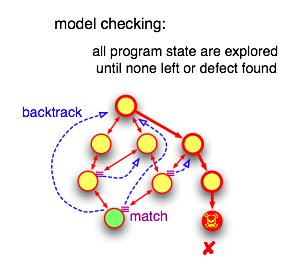
\includegraphics[scale=0.5]{figures/states-mc.png}
          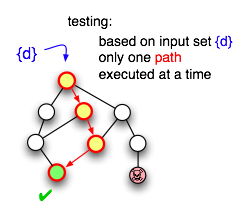
\includegraphics[scale=0.6]{figures/states-testing.png}
      \end{center}
  \end{frame}
% --------------------------------------------------------------------------- %
  \begin{frame}{TLA+ -- Temporal Logic of Actions}
      \begin{center}
          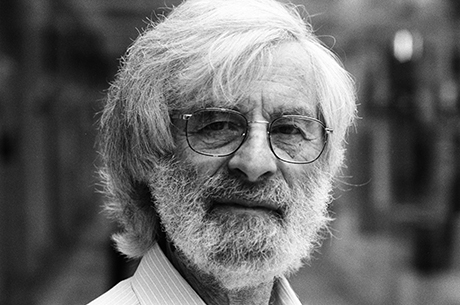
\includegraphics[scale=0.3]{figures/lamport.jpg}
      \end{center}
      \textbf{TLA+} language developed by \textbf{Leslie Lamport}. It is
      used to design, model, document, and verify concurrent systems, has
      been described as exhaustively-testable pseudocode and blueprints
      for software systems.
  \end{frame}
% --------------------------------------------------------------------------- %
  \begin{frame}{TLA+ industry usage: AWS}
    \begin{center}
       
\includegraphics[scale=0.08]{figures/aws}
    \end{center}
      \textbf{TLA+} helped to find design bugs in \textbf{S3, Dynamo, EBS, EC2},
      etc, some requiring traces of 35 steps.~\cite{aws2014}
  \end{frame}
% --------------------------------------------------------------------------- %
  \begin{frame}{TLA+ industry usage: Microsoft}
      MS used TLA+ to define consistency protocol for CosmosDB and memory
      allocator for XBox~\cite{ms2017}
    \begin{center}
        
\includegraphics[scale=0.2]{figures/cosmos}
    \end{center}
    \begin{center}
        
\includegraphics[scale=0.2]{figures/xbox}
    \end{center}
  \end{frame}
% --------------------------------------------------------------------------- %
  \begin{frame}{TLA+ industry usage: Opens source}
      Number open source projects use TLA+ to verify complex algorithms:
    \begin{itemize}
        \item Elastic -- data replication protocol~\cite{elastic2017}
        \item Mongodb -- data replication protocol~\cite{mongo2016}
        \item Hadoop/YARN -- registry of long lived processes~\cite{hadoop2017}
    \end{itemize}
    \begin{center}
        
\includegraphics[scale=0.1]{figures/mongo}
        
\includegraphics[scale=0.12]{figures/elastic}
        
\includegraphics[scale=0.14]{figures/hadoop}
    \end{center}
  \end{frame}
% --------------------------------------------------------------------------- %
  \section{TLA+ Basics}
% --------------------------------------------------------------------------- %
  \begin{frame}{TLA+ hello worlds}
    \begin{center}
      \inputminted[linenos,fontsize=\scriptsize]{tla}{figures/hourclock.tla}
      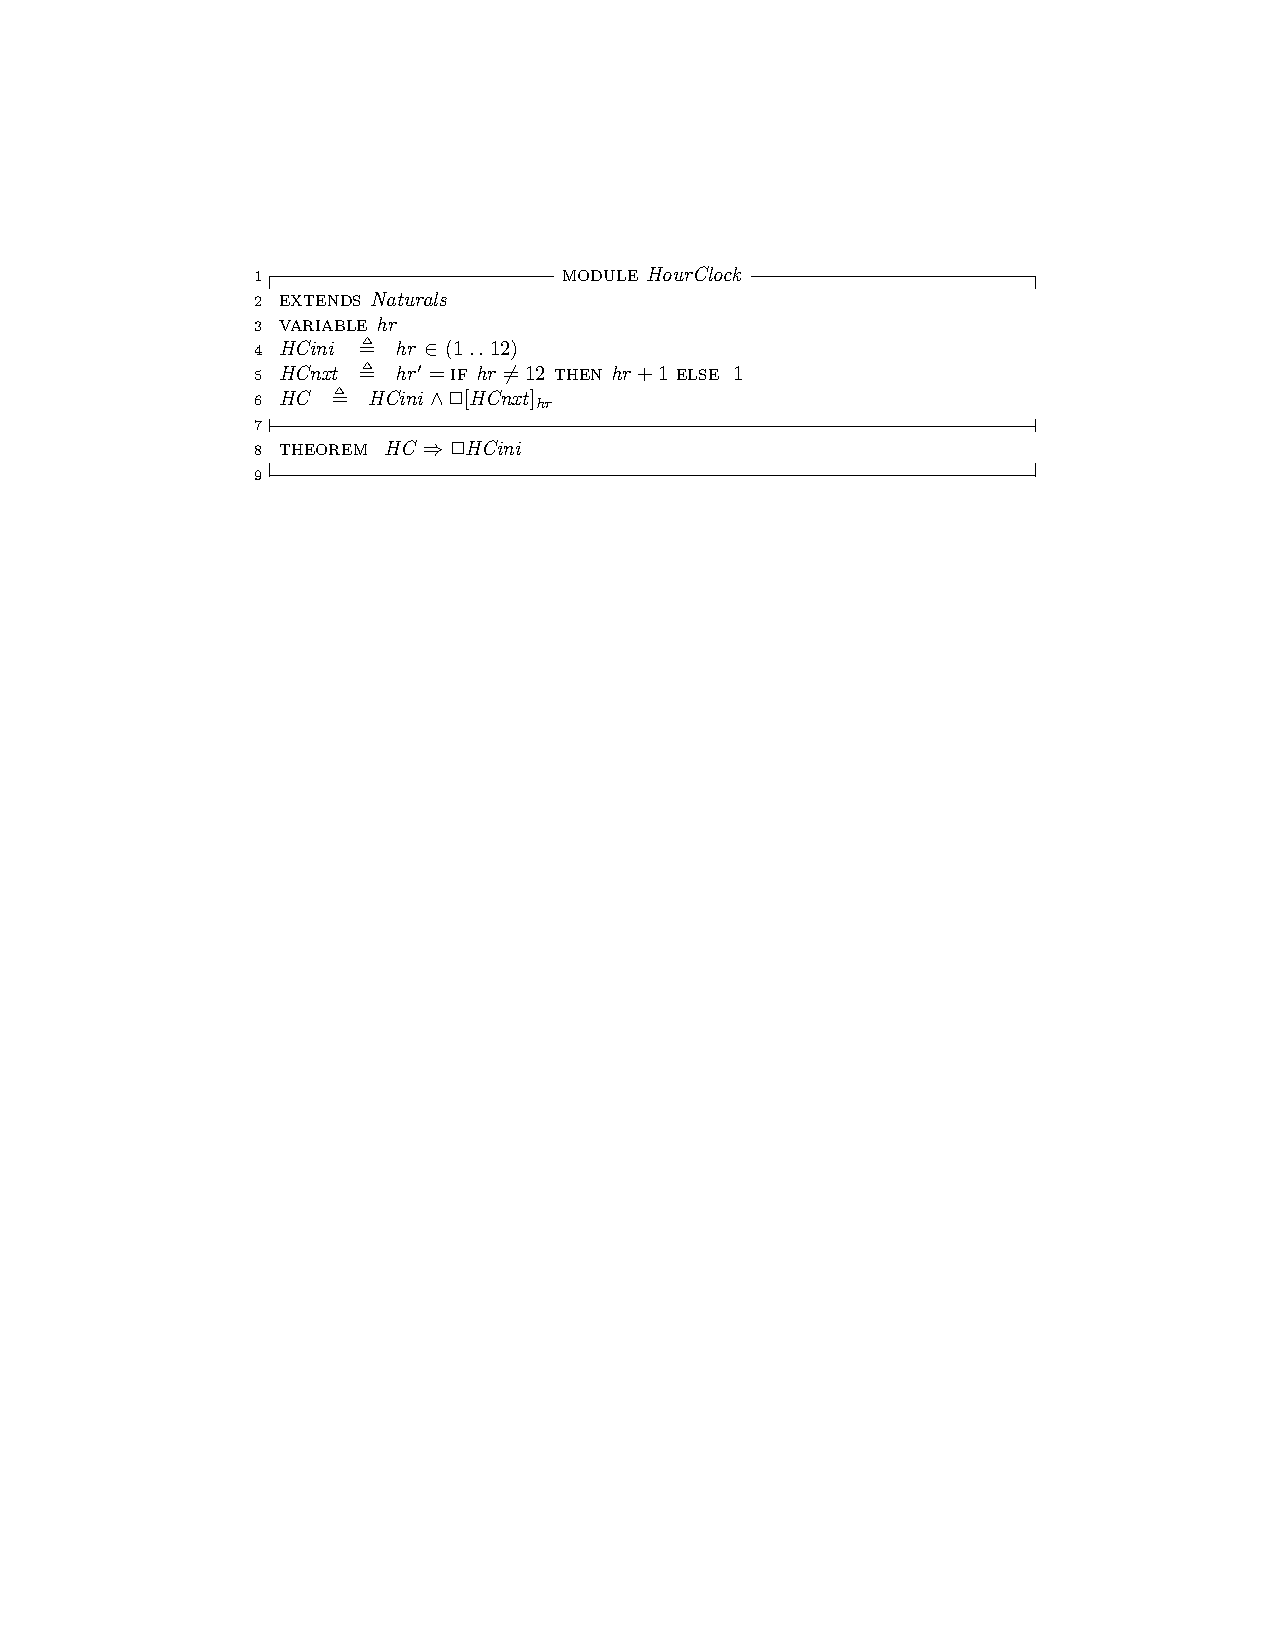
\includegraphics[scale=0.8]{figures/hourclock.pdf}
    \end{center}
  \end{frame}
% --------------------------------------------------------------------------- %
  \begin{frame}{TLA+ syntax. Logic}
      Basic logical operators:
      \begin{description}
        \item[$\lor$] logical OR, $or$ in python
        \item[$\land$] logical AND, $and$ and in python
        \item[$\lnot$] logical NOT, $and$ and in python
        \item[$=$] boolean operator, checks equality, it is not an assignment operator.
        \item[$\triangleq$] boolean operator, checks equality, it is not an assignment operator.
      \end{description}
  \end{frame}
% --------------------------------------------------------------------------- %
  \begin{frame}{TLA+ syntax. More Logic}
      More logic operators:
      \begin{description}
        \item[$\exists$] means "there exists", written as E in ASCII
        \item[$\forall$]  means "for all", written as A in ASCII
        \item[$:$] colon reads as "such that"
      \end{description}
      $\exists x \in {1,2,3,4,5} : x > 3$ - exists $x$ in
      set of integers ${1,2,3,4,5}$ such that $x > 3$ expression evaluates
      to TRUE.
  \end{frame}
% --------------------------------------------------------------------------- %
  \begin{frame}{TLA+ syntax. More Logic}
      More logic operators:
      \begin{description}
        \item[$\square$] formula is TRUE on each step
        \item[$\Diamond$] eventually TRUE
        \item[$\implies$] logical implication
        \item[$'$] reads as prime, state of variable on next step

      \end{description}
      $\exists x \in {1,2,3,4,5} : x > 3$~-- exists $x$ in
      set of integers ${1,2,3,4,5}$ such that $x > 3$ expression evaluates to TRUE.
  \end{frame}
% --------------------------------------------------------------------------- %
  \begin{frame}{TLA+ Spec Template}
      \begin{center}
          \inputminted[linenos, fontsize=\scriptsize]{tla}{figures/template.tla}
      \end{center}
  \end{frame}
% --------------------------------------------------------------------------- %
  \section{Aiorwlock Spec}
% --------------------------------------------------------------------------- %
  \begin{frame}[fragile]{aiorwlock~-- read write lock for asyncio}
      An RW lock allows concurrent access for read-only operations,
      while write operations require exclusive access, simple example:
      \inputminted[linenos,fontsize=\scriptsize]{python}{figures/lock.py}
  \end{frame}
% --------------------------------------------------------------------------- %
  \begin{frame}{aiorwlock~-- bug}
      \begin{center}
        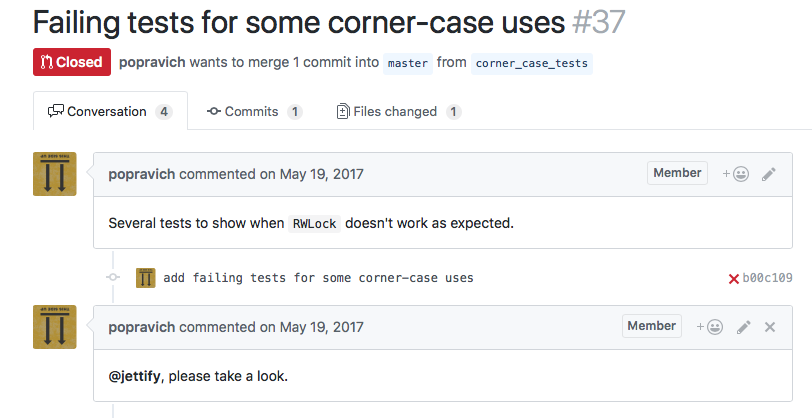
\includegraphics[scale=0.40]{figures/aiorwlock_bug}
      \end{center}
  \end{frame}
% --------------------------------------------------------------------------- %
  \begin{frame}{aiorwlock possible states}
      Read Write lock state machine:
      \begin{center}
          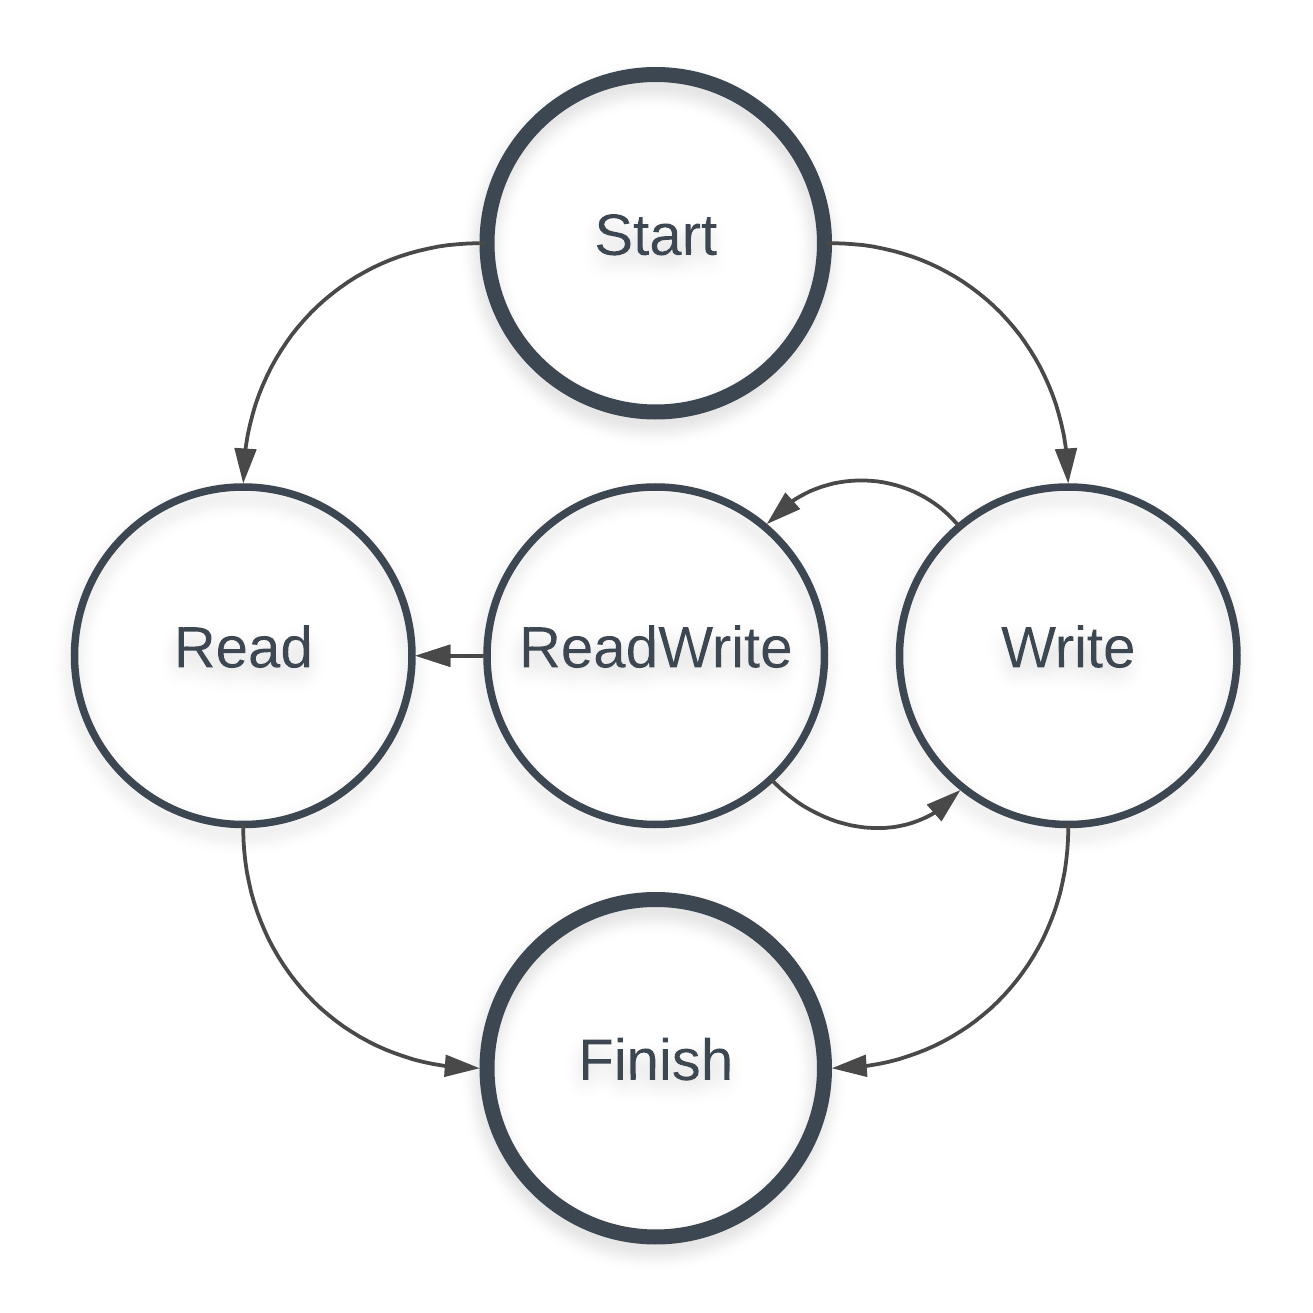
\includegraphics[scale=0.15]{figures/task_states2}
      \end{center}
  \end{frame}
% --------------------------------------------------------------------------- %
  \begin{frame}{aiorwlock implementation sketch}
      Full implementation available in~\cite{jettify2016}
      \begin{center}
          \inputminted[linenos,fontsize=\scriptsize]{python}{figures/read.py}
      \end{center}
  \end{frame}
% --------------------------------------------------------------------------- %
  \begin{frame}{aiorwlock TLA spec: part 1}
      \begin{center}
          \inputminted[firstline=1,lastline=19,linenos,
            fontsize=\scriptsize]{tla}{figures/aiorwlock.tla}
      \end{center}
  \end{frame}
% --------------------------------------------------------------------------- %
  \begin{frame}{aiorwlock TLA spec: part 2}
      \begin{center}
          \inputminted[firstline=20,lastline=31,linenos,
            fontsize=\scriptsize]{tla}{figures/aiorwlock.tla}
      \end{center}
  \end{frame}
% --------------------------------------------------------------------------- %
  \begin{frame}{aiorwlock TLA spec: part 3}
      \begin{center}
          \inputminted[firstline=34,lastline=47,linenos,
            fontsize=\scriptsize]{tla}{figures/aiorwlock.tla}
      \end{center}
  \end{frame}
% --------------------------------------------------------------------------- %
  \begin{frame}{aiorwlock TLA spec: part 4}
      \begin{center}
          \inputminted[firstline=47,lastline=58,linenos,
            fontsize=\scriptsize]{tla}{figures/aiorwlock.tla}
      \end{center}
  \end{frame}
% --------------------------------------------------------------------------- %
  \begin{frame}{aiorwlock possible states}
      \begin{center}
          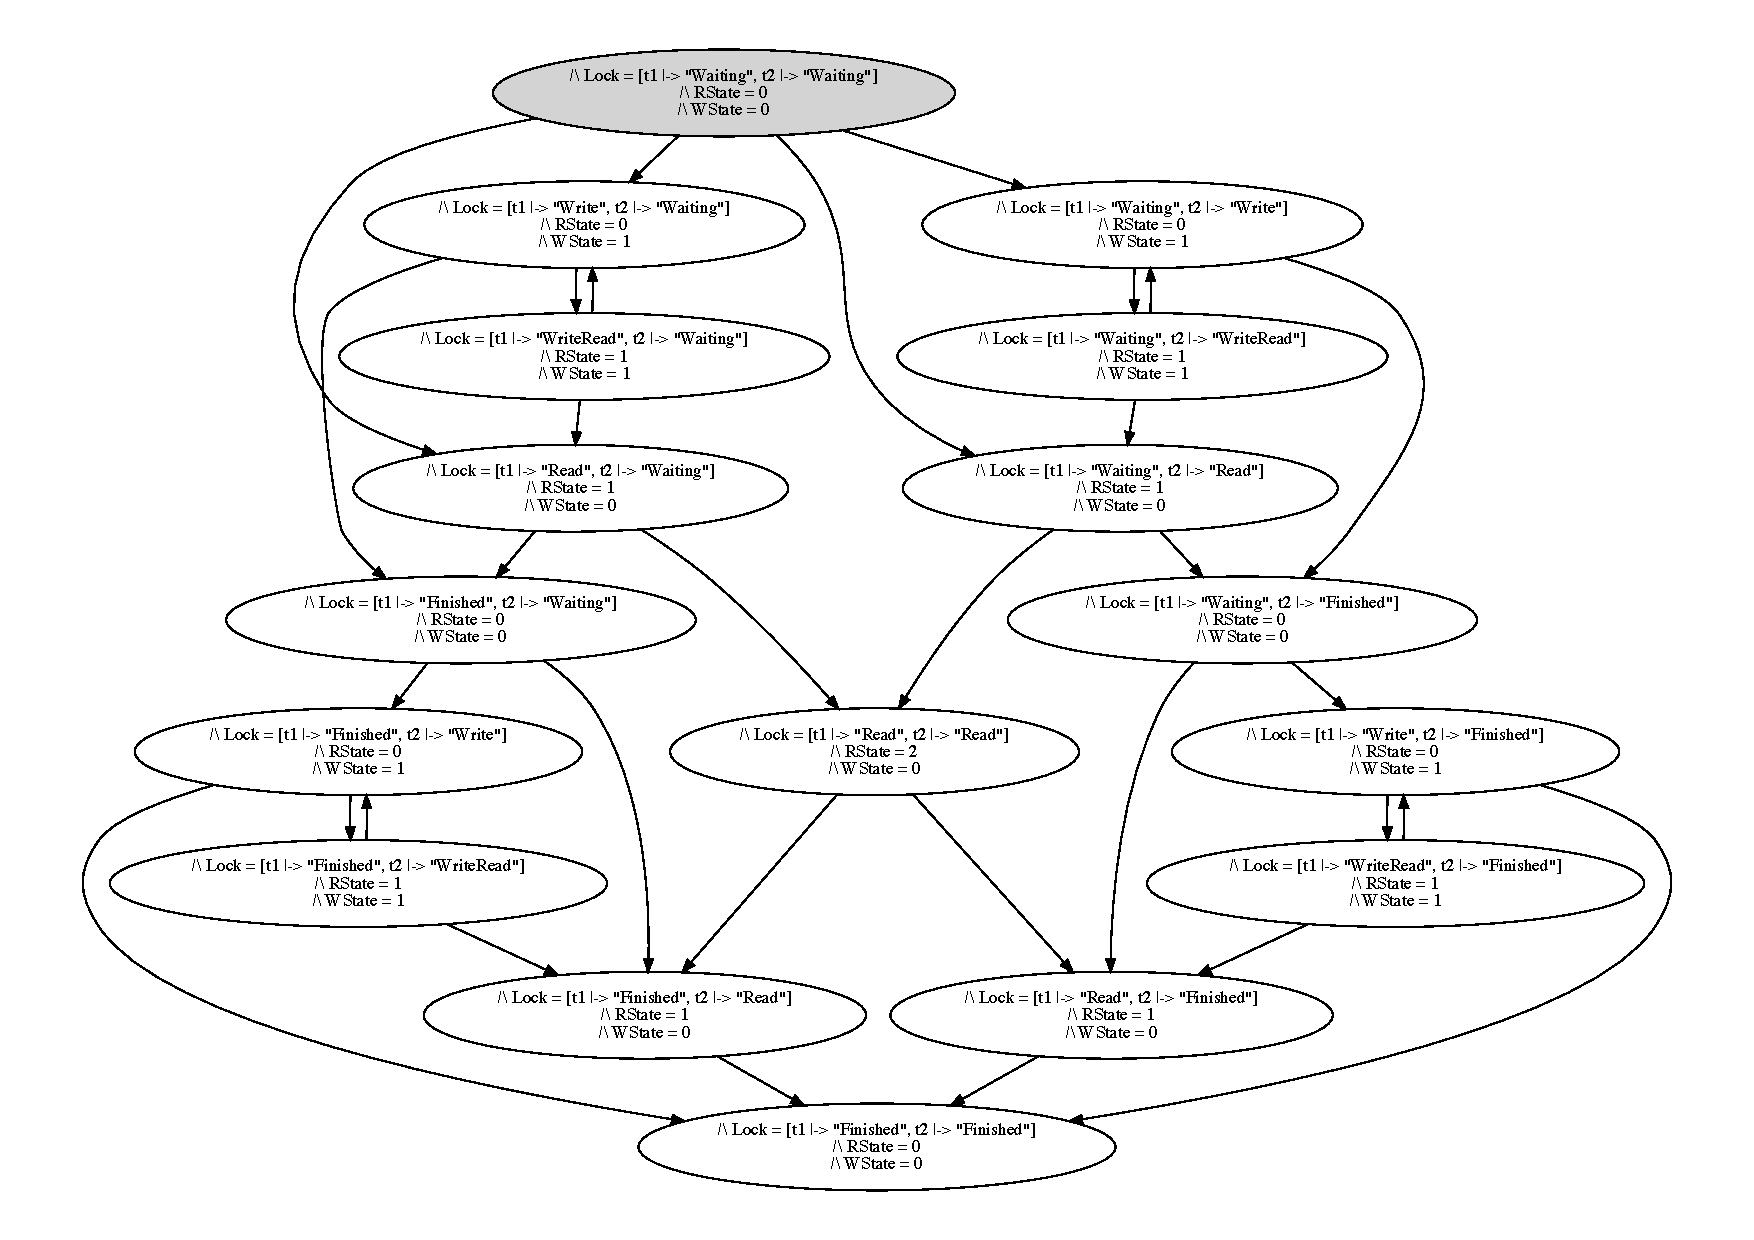
\includegraphics[scale=0.35,angle=90]{figures/aiorwlock_model}
      \end{center}
  \end{frame}
% --------------------------------------------------------------------------- %
  \begin{frame}{aiorwlock trace}
      TLC shows all steps that leads to \textit{invariant violation}.
      \begin{center}
          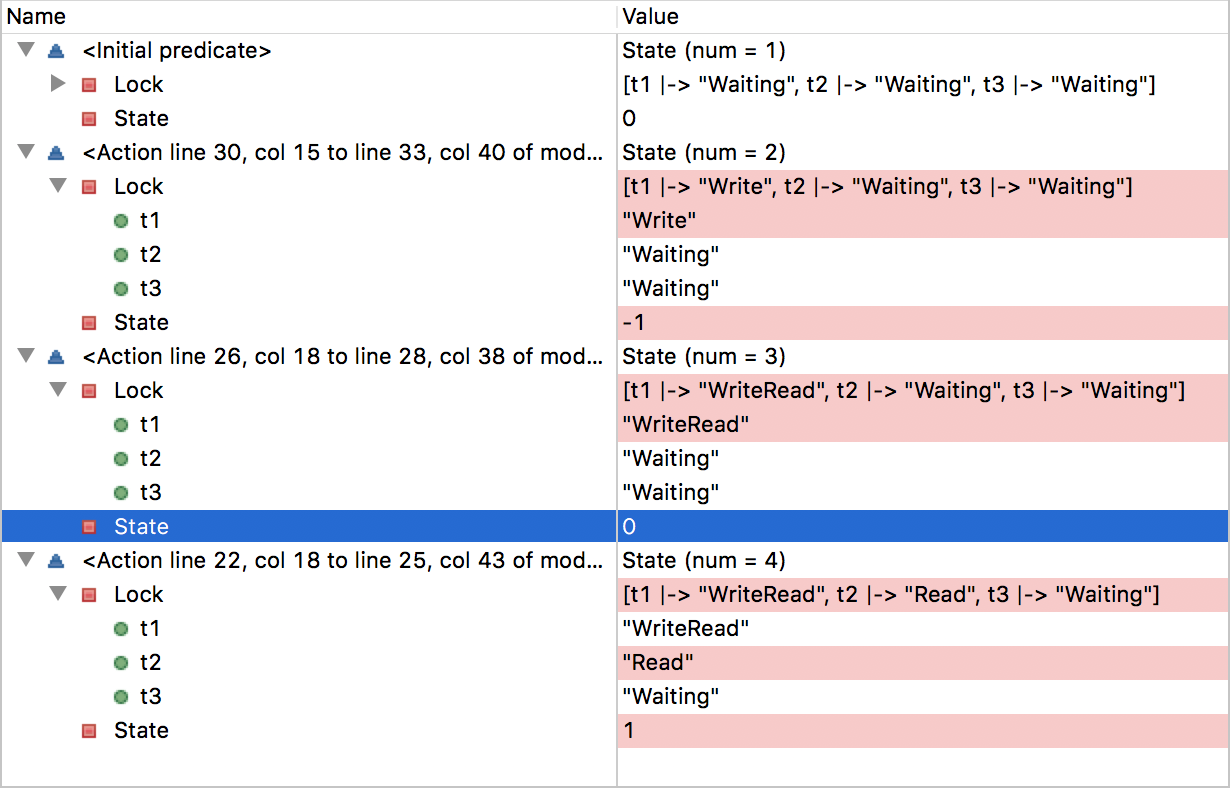
\includegraphics[scale=0.45]{figures/tla_trace}
      \end{center}
  \end{frame}
% --------------------------------------------------------------------------- %
  \begin{frame}{aiorwlock spec results}
    \begin{itemize}
      \item In fact bug reveled itself on specification phase, before
          running any models
      \item Only three steps required to reproduce issue
    \end{itemize}
  \end{frame}
% --------------------------------------------------------------------------- %
  \section{Multithreading Queue Spec}
% --------------------------------------------------------------------------- %
  \begin{frame}{Multithreading Queue}
      Classic \textit{bounded buffer}, attempts to put an element into a
      full queue or take from empty will block.
      \begin{center}
          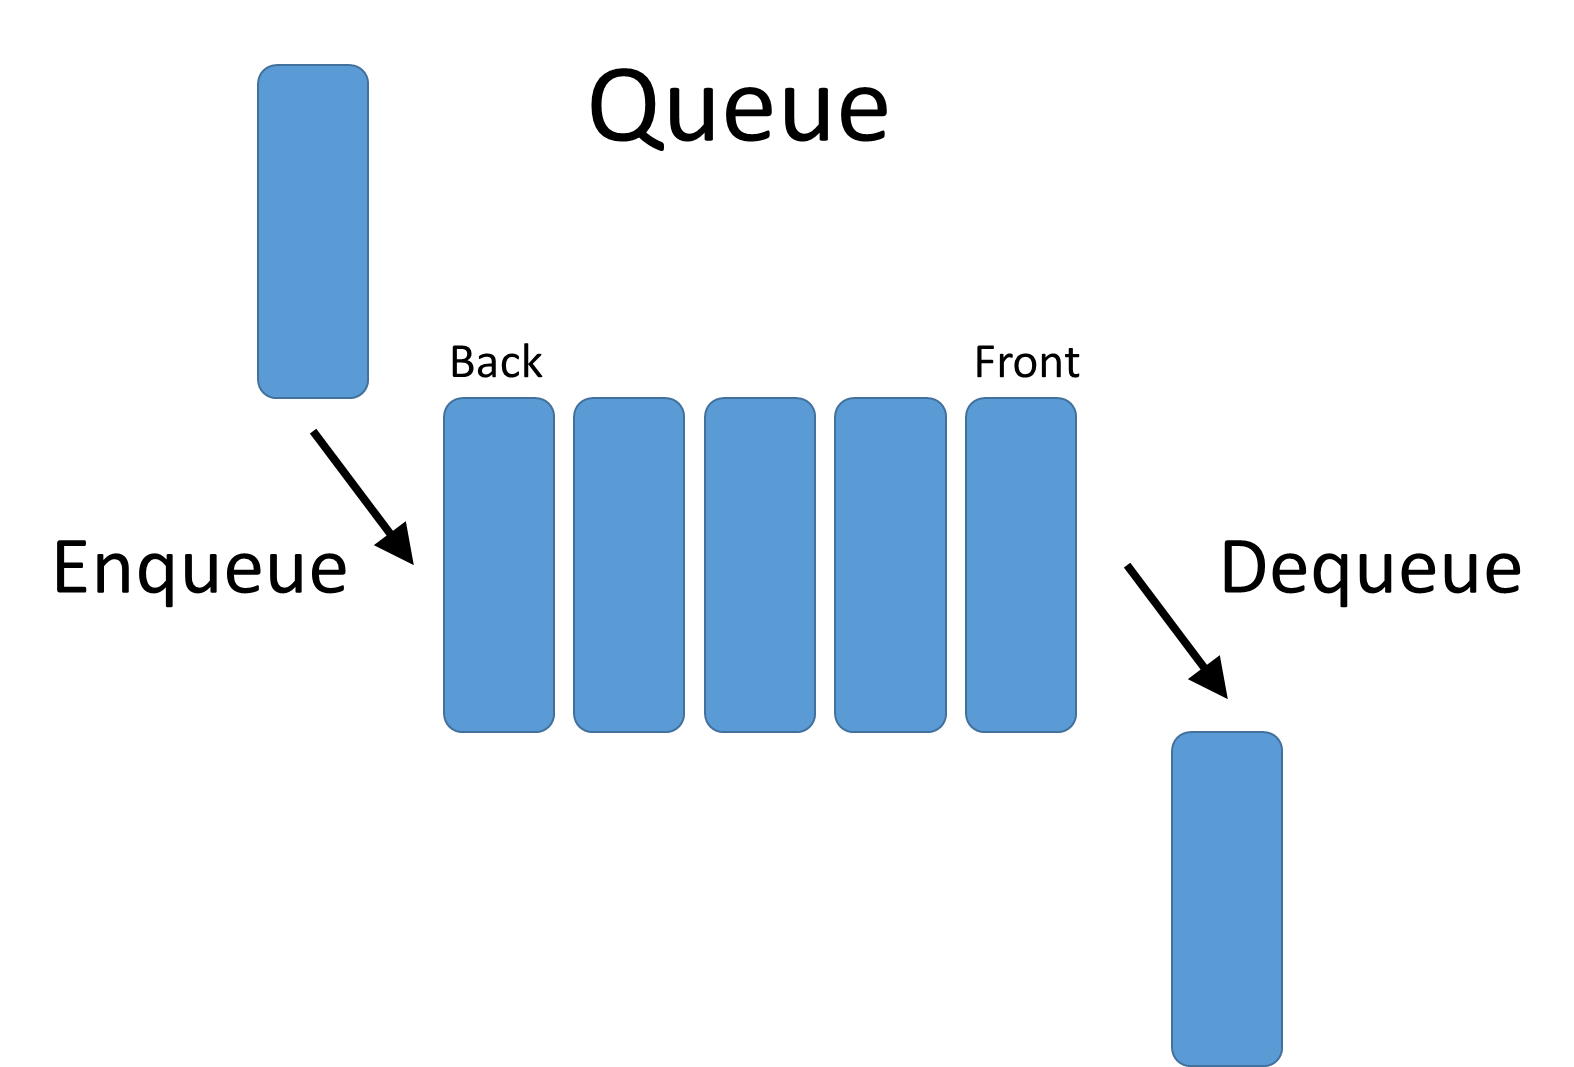
\includegraphics[scale=0.30]{figures/queue}
      \end{center}
  \end{frame}
% --------------------------------------------------------------------------- %
  \begin{frame}{Queue implementation, part 1}
      \begin{center}
          \inputminted[firstline=1,lastline=20,linenos,
            fontsize=\scriptsize]{python}{figures/queue.py}
      \end{center}
  \end{frame}
% --------------------------------------------------------------------------- %
  \begin{frame}{Queue implementation, part 2}
      \begin{center}
          \inputminted[firstline=22,lastline=40,linenos,
            fontsize=\scriptsize]{python}{figures/queue.py}
      \end{center}
  \end{frame}
% --------------------------------------------------------------------------- %
  \begin{frame}{Queue TLA spec: part 1}
      \begin{center}
          \inputminted[firstline=1,lastline=16,linenos,
            fontsize=\scriptsize]{tla}{figures/buffer.tla}
      \end{center}
  \end{frame}
% --------------------------------------------------------------------------- %
  \begin{frame}{Queue TLA spec: part 2}
      \begin{center}
          \inputminted[firstline=16,lastline=31,linenos,
            fontsize=\scriptsize]{tla}{figures/buffer.tla}
      \end{center}
  \end{frame}
% --------------------------------------------------------------------------- %
  \begin{frame}{Queue TLA spec: part 3}
      \begin{center}
          \inputminted[firstline=32,lastline=50,linenos,
            fontsize=\scriptsize]{tla}{figures/buffer.tla}
      \end{center}
  \end{frame}
% --------------------------------------------------------------------------- %
  \begin{frame}{Multithreading Queue Spec Results}
    \begin{itemize}
      \item In fact bug reveled itself on specification phase, before running any models
      \item More than \textbf{40 steps} required to reproduce deadlock!
      \item Thread programming is hard!
    \end{itemize}
  \end{frame}
% --------------------------------------------------------------------------- %
  \begin{frame}{Queue trace}
      TLC shows all steps that leads to \textit{invariant violation}.
      \begin{center}
          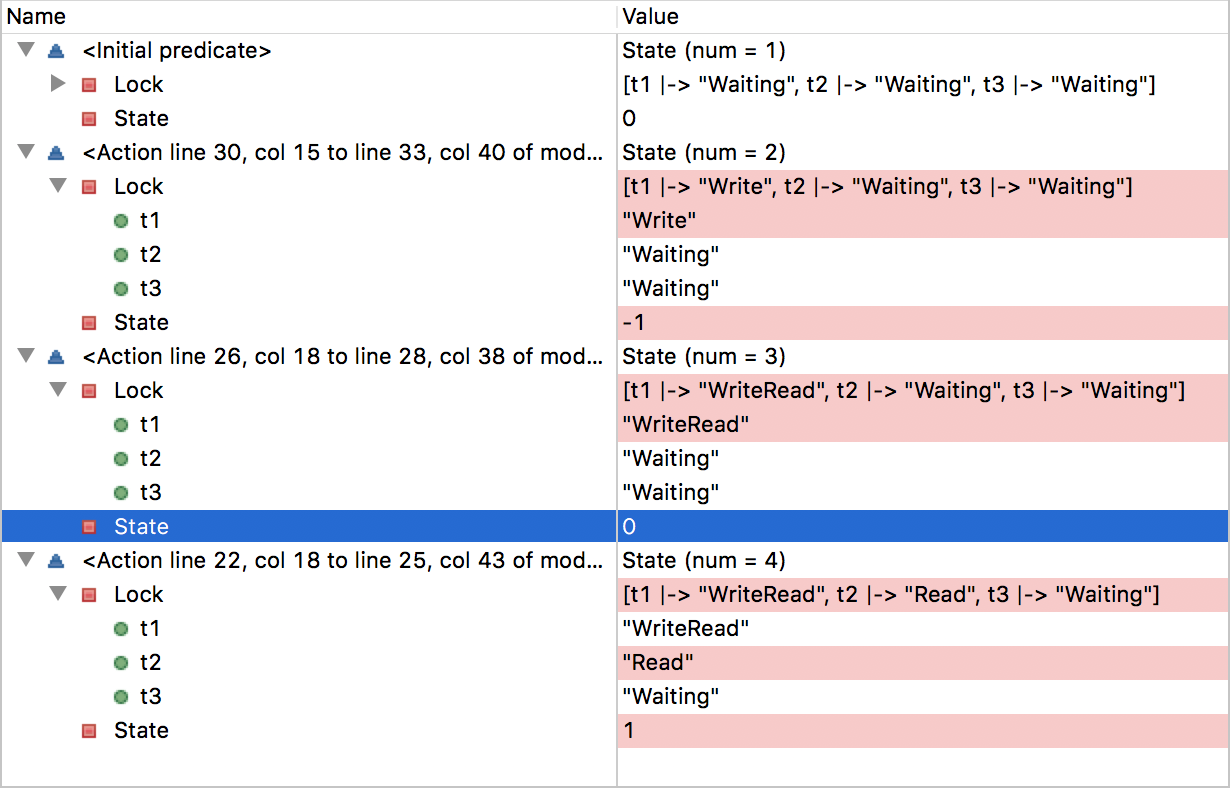
\includegraphics[scale=0.45]{figures/tla_trace}
      \end{center}
  \end{frame}
% --------------------------------------------------------------------------- %
  \section{Conclusions}
% --------------------------------------------------------------------------- %
  \begin{frame}{Limitations of Model-Checking}
    \begin{itemize}
      \item State space explosion number of states reachable by a system
          can quickly become huge, or even infinite
      \item Used as an adjunct to, not a replacement for, standard quality
          assurance methods
      \item Formal methods are not a panacea, but can increase confidence in
          a product’s reliability if applied with care and skill
      \item Very useful for consistency checks, but can not assure completeness
    \end{itemize}
  \end{frame}
% --------------------------------------------------------------------------- %
\begin{frame}
    \vspace{1cm}
    \begin{center}{\Huge Questions?} \end{center}
    \begin{center} 
\includegraphics[scale=0.7]{figures/qrcode}\end{center}
    \begin{center}
        \href{http://github.com/jettify}{http://github.com/jettify}
    \end{center}
\end{frame}
% --------------------------------------------------------------------------- %
\appendix
\begin{frame}[allowframebreaks]{References}
    \bibliography{references}
    \bibliographystyle{abbrv}
\end{frame}
% --------------------------------------------------------------------------- %
\end{document}
% =========================================================================== %
